\documentclass[a4paper,UTF8]{ctexart}
%\documentclass[a4paper,UTF8]{ctexrep}
\ctexset{
    section={
        name={,、},
        aftername={},
        number=\chinese{section},
        format+={\raggedright},
    },
    subsection={
        name={(,)},
        aftername={},
        number=\chinese{subsection},
        indent=1\ccwd,
    },
}

\usepackage{lipsum}
\usepackage{fancyhdr}
\pagestyle{empty}
%\usepackage{xeCJK}
\usepackage{caption}
\usepackage[a4paper, margin={3.18cm, 2.54cm}]{geometry}
\usepackage[T1]{fontenc}
\usepackage{float}
\usepackage[newfloat]{minted}
\usepackage{mdframed}
\usepackage{hyperref}
\hypersetup{
    colorlinks=false,
    linktoc=all,
}
%\usepackage[chinese, provide=*]{babel}
\usepackage{graphicx}
\graphicspath{{images/}}

\setminted{baselinestretch=1}
\SetupFloatingEnvironment{listing}{name=代码,placement=h}
%\renewcommand\figurename{\heiti 图}
%\renewcommand\tablename{\heiti 表}
\renewcommand{\theFancyVerbLine}{{\arabic{FancyVerbLine}}}
\iffalse
\captionsetup{
%    width=0.9\linewidth, % width of caption is 90% of current textwidth
    labelfont=bf,        % the label, e.g. figure 12, is bold
    font=small,          % the whole caption text (label + content) is small
}
\fi

\iffalse
\newmintedfile[cppcode]{cpp}{
    fontfamily=tt,
    linenos=true,
    numberblanklines=true,
    numbersep=5pt,
    gobble=0,
    frame=leftline,
    framerule=0.4pt,
    framesep=2mm,
    funcnamehighlighting=true,
    tabsize=4,
    obeytabs=false,
    mathescape=false,
    samepage=false,
    showspaces=false,
    showtabs=false,
    texcl=false,
    breaklines=true,
    stripnl=true,
}
\fi
\newcommand{\cppcode}[1]{{
    \CJKsetecglue{}
    \inputminted[
    frame=single,
    framesep=2mm,
    fontsize=\footnotesize,
    tabsize=4,
    samepage=false,
    breaklines=true,
    stripnl=true,
    formatcom=\heiti,
    linenos=true]{cpp}{#1}
}}
\newcommand{\textcode}[1]{{
    \CJKsetecglue{}
    \inputminted[
    frame=single,
    framesep=2mm,
    fontsize=\footnotesize,
    tabsize=4,
    samepage=false,
    breaklines=true,
    breakanywhere=true,
    stripnl=false,
    linenos=false]{text}{#1}
}}
\setlength\partopsep{-\topsep}

\setCJKfamilyfont{hwxk}{STXingkai}               %华文行楷  hwxk
\newcommand{\hwxk}{\CJKfamily{hwxk}}
\setmainfont{Times New Roman}

\begin{document}

\begin{titlepage}
\newgeometry{margin={1in,1.5in}}
\center{\Huge\hwxk **REDACTED**}
\vspace{6cm}
\center{\fontsize{32pt}{\baselineskip}\selectfont\kaishu{数据结构课程设计}}
\vspace{6cm}

\begin{tabular}{l c}
    \LARGE{\heiti 班级}& \hspace{1.7cm}\LARGE\heiti **REDACTED**\hspace{1.7cm} \\
    \cline{2-2}\\
    \LARGE{\heiti 学号}& \hspace{1.7cm}\LARGE\heiti **REDACTED**\hspace{1.7cm} \\
    \cline{2-2}\\
    \LARGE{\heiti 姓名}& \LARGE\heiti **REDACTED**\\
    \cline{2-2}\\
    \LARGE{\heiti 指导教师}& \LARGE\heiti **REDACTED**\\
    \cline{2-2}
\end{tabular}
\restoregeometry
\end{titlepage}
\newpage

\tableofcontents
\newpage

\section{菜鸟智慧系统}
\subsection{数据结构}
使用的数据结构为双向链表。
\subsection{算法设计思想}
将货架中的包裹作为链表节点的数据,包裹的上架与取出对应着链表节点的加入与移除。包裹编号通过遍历链表并定位空缺的编号来实现。包裹在货架上需要有序排放,对应着链表的排序,此代码中使用自底向上的归并排序实现。文件以 JSON 格式保存了系统的状态,保证了清晰与直观。
\subsection{源程序}
\cppcode{../代码/01-菜鸟智慧系统/main.cpp}
{\captionof{listing}{main.cpp}}
\cppcode{../代码/01-菜鸟智慧系统/json.h}
{\captionof{listing}{json.h}}
\cppcode{../代码/01-菜鸟智慧系统/json.cpp}
{\captionof{listing}{json.cpp}}
\cppcode{../代码/01-菜鸟智慧系统/hashmap.h}
{\captionof{listing}{hashmap.h}}
\cppcode{../代码/01-菜鸟智慧系统/hashmap.cpp}
{\captionof{listing}{hashmap.cpp}}
\subsection{测试数据及结果}
可能的交互如下:
\textcode{./interactions/01-01.txt}
生成的文件如下:
\textcode{./interactions/01-02.txt}
\subsection{时间复杂度}
时间复杂度为 $O(n)$。
\subsection{问题及可改进的点}
可以为系统添加更多统计、管理等功能。

\section{算术表达式求值}
\subsection{数据结构}
使用的数据结构为栈。
\subsection{算法设计思想}
逐个对字符串中的字符进行判断,若为符号则根据优先级判断是否要处理栈内已有的数据,然后入运算符栈;若为数字则调用贪婪的字符串转浮点数函数,入操作数栈。其中括号需要做特殊处理,以便进行计算与错误定位。由于只有二元运算符,因此在每次入栈前,代码都会检查相邻的记号是否亲和(如加号只能与数字或括号亲和),并对有问题的组合报错。当读取到第二个 \# 时处理栈中剩余的所有符号,以确定是否存在不匹配的括号等错误。
\subsection{源程序}
\cppcode{../代码/02-算术表达式求值/main.cpp}
{\captionof{listing}{main.cpp}}
\subsection{测试数据及结果}
可能的交互如下:
\textcode{./interactions/02-01.txt}
\subsection{时间复杂度}
时间复杂度为 $O(n)$。
\subsection{问题及可改进的点}
代码只对二元运算符做了支持,还可以加入一元、三元等运算符的支持。

\section{特殊路径统计}
\subsection{数据结构}
使用的数据结构为树、栈。
\subsection{算法设计思想}
通过路径栈获得两个节点的共同最近祖先,从而确定两个节点之间的简单路径,并通过判断路径上的所有节点来确定是否为特殊路径。暴力枚举所有节点的组合对,从而统计出总共的特殊路径个数。
\subsection{源程序}
\cppcode{../代码/03-特殊路径统计/main.cpp}
{\captionof{listing}{main.cpp}}
\subsection{测试数据及结果}
\begin{verbatim}
[样例 1]
输入:
7
0 5 5 1 4 1 4
输出:
10
[样例 2]
输入:
5
2 3 0 2 2
输出:
7
\end{verbatim}
\subsection{时间复杂度}
时间复杂度为 $O(n^2\log n)$。
\subsection{问题及可改进的点}
算法的效率过低,可考虑改进算法。

\section{公交线路提示}
\subsection{数据结构}
使用的数据结构为邻接表、栈、队列。
\subsection{算法设计思想}
转车次数最少的乘车路线通过 BFS 求出(每一步都将所有未访问过的公交路线加入队列)。经过站点最少的乘车路线通过 Dijkstra 求出。路线的最终构建通过栈来实现。
\subsection{源程序}
\cppcode{../代码/04-公交线路提示/main.cpp}
{\captionof{listing}{main.cpp}}
\subsection{测试数据及结果}
可能的交互如下:
\textcode{./interactions/04-01.txt}
\subsection{时间复杂度}
代码中 Dijkstra、BFS 的时间复杂度分别为 $O((V+E)*V)$、$O(V+E^2)$。
\subsection{问题及可改进的点}
Dijkstra 的时间复杂度可以通过优先队列等方式进一步优化;BFS 的时间复杂度也不够理想,通过额外增加路线的存储信息可以将其优化到标准时间复杂度 $O(V+E)$。

\section{Huffman 编码与解码}
\subsection{数据结构}
使用的数据结构为 Huffman 树。
\subsection{算法设计思想}
通过优先队列建树,总共为 0-256 共 257 个可能的值(一个字节的所有取值 + 结束符)进行编码。编码时从树生成每种取值对应的 Huffman 码表示并写入比特,最后写入结束符;解码时通过读取的比特访问树上结点,直至到达数据结点,获得实际数据,或者是读取到代表结束的 256,停止读取。
\subsection{源程序}
\cppcode{../代码/05-Huffman编码与解码/main.cpp}
{\captionof{listing}{main.cpp}}
\subsection{测试数据及结果}
可能的交互如下:
\textcode{./interactions/05-01.txt}
编码材料内容如下:
\textcode{./interactions/05-02.txt}
通过编码还原得到的文本与上面完全一致。\par
生成的统计信息如下:
\textcode{./interactions/05-03.txt}
\subsection{时间复杂度}
时间复杂度为 $O(n)$。
\subsection{问题及可改进的点}
目前程序性能较差,可在算法、基础设施等多个地方进行改进。

\section{排序算法比较}
\subsection{数据结构}
使用的数据结构为栈、链表。
\subsection{算法设计思想}
插入排序:将新的元素插入到旧的有序列表中的合适位置,使得生成的新列表仍然有序,直到所有元素都已插入。\par
希尔排序:类似插入排序,通过在插入排序之前使用特定递减的步长序列对元素进行分组,并对每组元素进行插入排序来优化时间复杂度。\par
冒泡排序:从第一个元素开始,将其与后继元素比较,若前者大则交换两者顺序,然后比较第二个元素与第三个元素的大小并交换,直到到达列表末尾,此时最大的元素已到达末尾。重复对除去最后一个元素后的子列表进行相同操作,直到子列表为空。\par
快速排序:通过分区函数将原列表分为三个部分(枢纽值(pivot),小于枢纽的列表(在原列表首部),大于枢纽的列表(在原列表尾部)),然后分别对新产生的列表进行相同操作,直到所有列表都已处理完毕。\par
选择排序:遍历列表,获取最小值,将其与列表中的第一个元素交换,然后对除去第一个元素以后的子列表进行相同操作,直到子列表为空。\par
堆排序:通过向下调整(sift down)实现对列表的就地堆化(变为大根堆),然后重复进行取出元素(至列表末尾)与调整二叉堆的操作,直到二叉堆为空。\par
归并排序:将列表二分,对每个新划分的列表进行归并排序,然后通过合并两个有序列表的方式得到最终的有序列表。\par
基数排序:按照十进制对元素进行每一位的划分,从最低位开始,使用计数排序(或任意稳定的排序)对列表进行一次排序,直到最高位排序完毕。
\subsection{源程序}
\cppcode{../代码/06-排序算法比较/main.cpp}
{\captionof{listing}{main.cpp}}
\subsection{测试数据及结果}
可能的交互如下:
\textcode{./interactions/06-01.txt}
\subsection{时间复杂度}
各算法的时间复杂度如下表所示:
\begin{table}[H]
\centering
\begin{tabular}{|l|l|}
    \hline
    插入排序 & $O(n^2)$ \\
    \hline
    希尔排序 & $O(n^{1.5})$ \\
    \hline
    冒泡排序 & $O(n^2)$ \\
    \hline
    快速排序 & $O(n\log n)$ \\
    \hline
    选择排序 & $O(n^2)$ \\
    \hline
    堆排序 & $O(n\log n)$ \\
    \hline
    归并排序 & $O(n\log n)$ \\
    \hline
    基数排序 & $O(dn)$ \\
    \hline
\end{tabular}
\end{table}
\subsection{问题及可改进的点}
无可改进的点。

\section{棋局评估}
\subsection{数据结构}
无使用的数据结构。
\subsection{算法设计思想}
通过 DFS 暴力枚举可能的局面,获取当前局面对当前下棋者的最佳得分。
\subsection{源程序}
\cppcode{../代码/08-棋局评估/main.cpp}
{\captionof{listing}{main.cpp}}
\subsection{测试数据及结果}
\begin{verbatim}
输入:
3
1 2 1
2 1 2
0 0 0
2 1 1
0 2 1
0 0 2
0 0 0
0 0 0
0 0 0
输出:
3
-4
0
\end{verbatim}
\subsection{时间复杂度}
时间复杂度为 $O(n^4)$,其中n为棋盘大小(3)。
\subsection{问题及可改进的点}
可考虑优化算法的时间复杂度。

\section{URL 映射}
\subsection{数据结构}
使用的数据结构为字符串。
\subsection{算法设计思想}
先将 URL 映射规则处理为易于处理的形式(分解为各种路径段),然后对于每个输入,枚举规则并尝试应用:若为完全匹配段,则确保字符串完全匹配;若为整数段,则匹配一串数字;若为字符串段,则匹配一段字符;若为路径段,则贪婪匹配剩余所有字符,最后校验斜杠等状态是否正确,若正确则输出。
\subsection{源程序}
\cppcode{../代码/10-URL映射/main.cpp}
{\captionof{listing}{main.cpp}}
\subsection{测试数据及结果}
\begin{verbatim}
输入:
5 4
/articles/2003/ special_case_2003
/articles/<int>/ year_archive
/articles/<int>/<int>/ month_archive
/articles/<int>/<int>/<str>/ article_detail
/static/<path> static_serve
/articles/2004/
/articles/1985/09/aloha/
/articles/hello/
/static/js/jquery.js
输出:
year_archive 2004
article_detail 1985 9 aloha
404
static_serve js/jquery.js
\end{verbatim}
\subsection{时间复杂度}
时间复杂度为 $O(n)$。
\subsection{问题及可改进的点}
可以考虑对字符串进行更深入的规格化,降低解析时的逻辑复杂度。

\section{词梯}
\subsection{数据结构}
使用的数据结构为邻接表、哈希表、队列。
\subsection{算法设计思想}
对于每个添加的单词,使它们连接至带有通配符的虚拟节点(如 work 连接至 *ork、w*rk、wo*k、wor*),以便在所有只相差一个字母的单词间建立联系,然后使用 BFS 进行查找。使用哈希表加速查找单词在图中对应的结点。
\subsection{源程序}
\cppcode{../代码/11-词梯/main.cpp}
{\captionof{listing}{main.cpp}}
\subsection{测试数据及结果}
可能的交互如下:
\textcode{./interactions/11-01.txt}
\subsection{时间复杂度}
时间复杂度为 $O(V+E)$。
\subsection{问题及可改进的点}
还可以考虑输出次优的词梯结果等。

\section{连连看}
\subsection{数据结构}
使用的数据结构为队列。
\subsection{算法设计思想}
通过 BFS 寻找并记录两点之间的所有关键点(起点、终点、转折点),通过检查关键点的总数来判断两点间是否可用小于等于 3 条直线相连,若可以则消除。
\subsection{源程序}
\cppcode{../代码/12-连连看/main.cpp}
{\captionof{listing}{main.cpp}}
\cppcode{../代码/12-连连看/res.h}
{\captionof{listing}{res.h}}
\cppcode{../代码/12-连连看/res.cpp}
{\captionof{listing}{res.cpp}}
\subsection{测试数据及结果}
以下为部分交互截图:
\begin{figure}[H]
\centering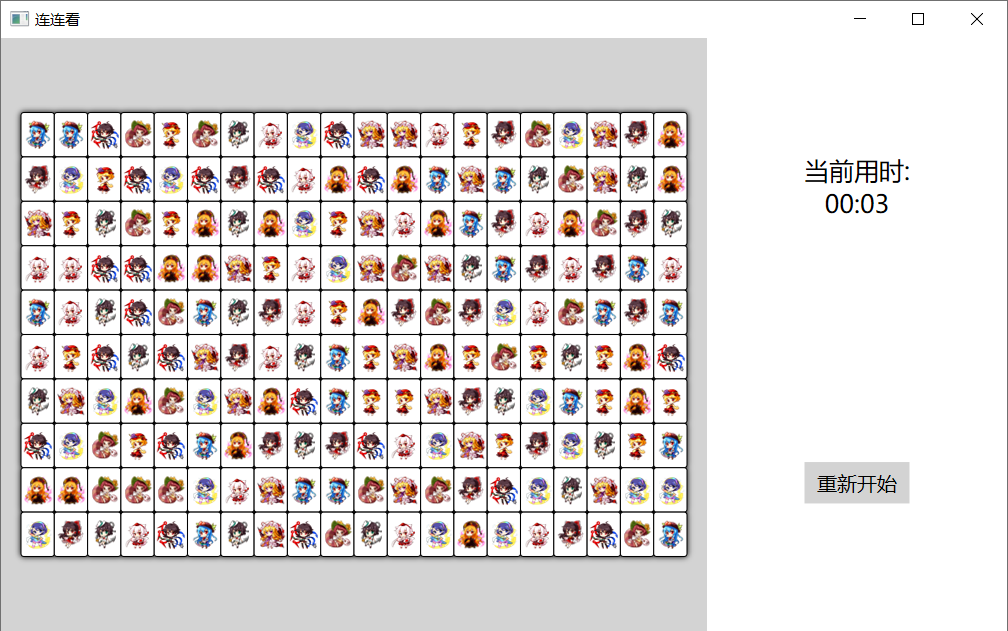
\includegraphics[width=\textwidth]{image01.png}\caption{初始状态}
\end{figure}
\begin{figure}[H]
\centering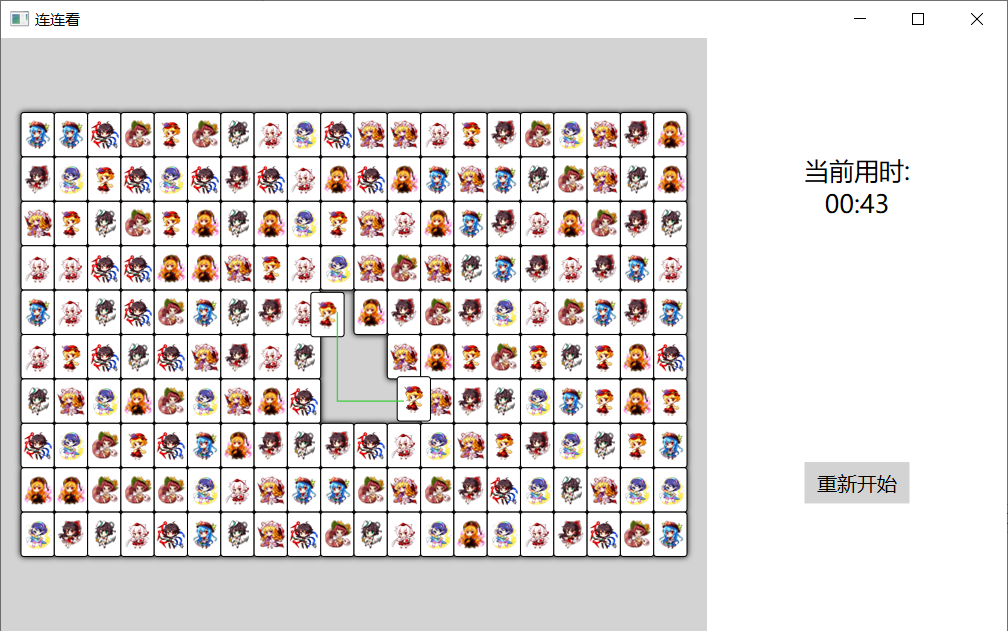
\includegraphics[width=\textwidth]{image02.png}\caption{消除成功}
\end{figure}
\begin{figure}[H]
\centering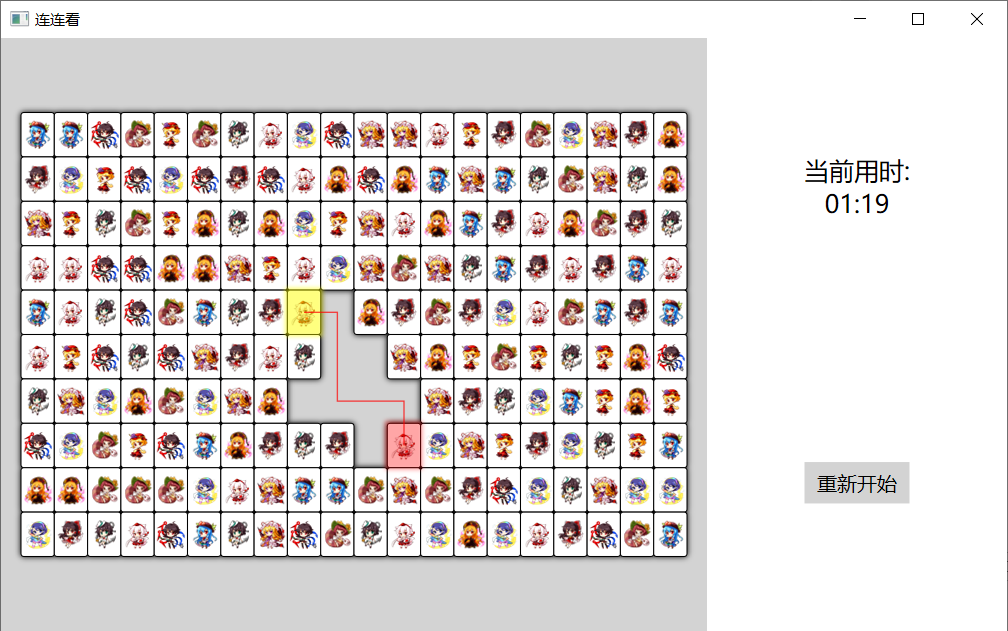
\includegraphics[width=\textwidth]{image03.png}\caption{消除失败}
\end{figure}
\subsection{时间复杂度}
时间复杂度为 $O(nm)$,其中 n、m 分别为局面的长、宽。
\subsection{问题及可改进的点}
代码的耦合度较高,可以考虑对代码结构进行优化。

\section{迷宫问题}
\subsection{数据结构}
使用的数据结构为栈、并查集。
\subsection{算法设计思想}
使用 DFS 从起点遍历所有相邻的可达路径(未访问过且非障碍物),若遇到终点则认为成功,否则直到栈空后认为没有可达路径。并查集用于 Kruskal 算法随机迷宫的生成。
\subsection{源程序}
\cppcode{../代码/15-迷宫问题/main.cpp}
{\captionof{listing}{main.cpp}}
\cppcode{../代码/15-迷宫问题/util.h}
{\captionof{listing}{util.h}}
\subsection{测试数据及结果}
以下为部分交互截图:
\begin{figure}[H]
\centering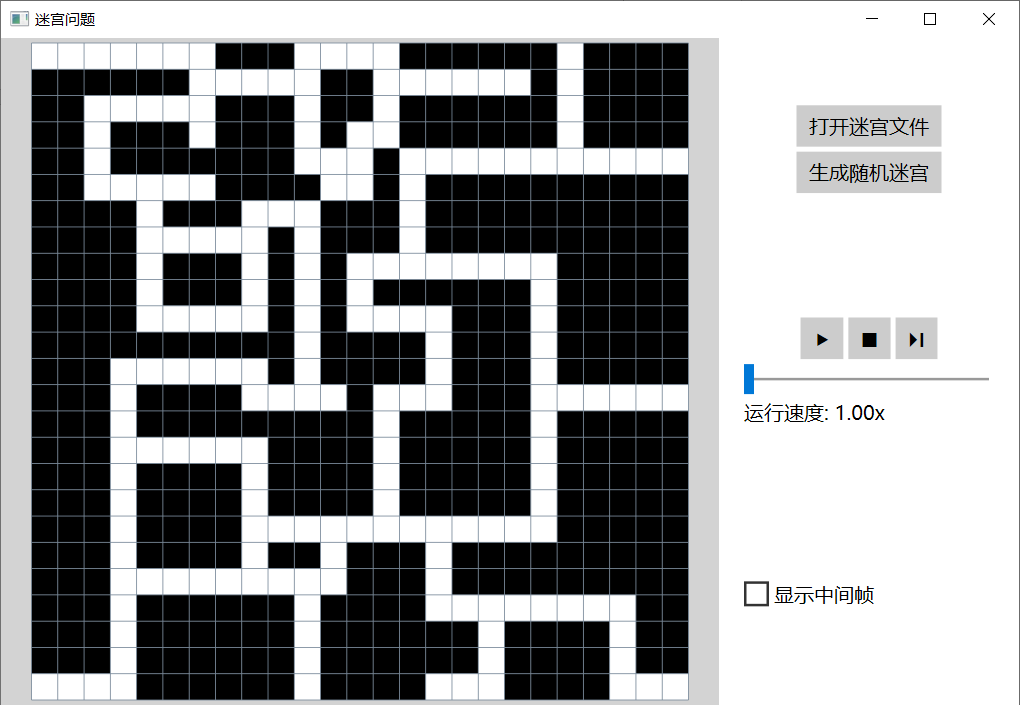
\includegraphics[width=\textwidth]{image04.png}\caption{加载迷宫文件}
\end{figure}
\begin{figure}[H]
\centering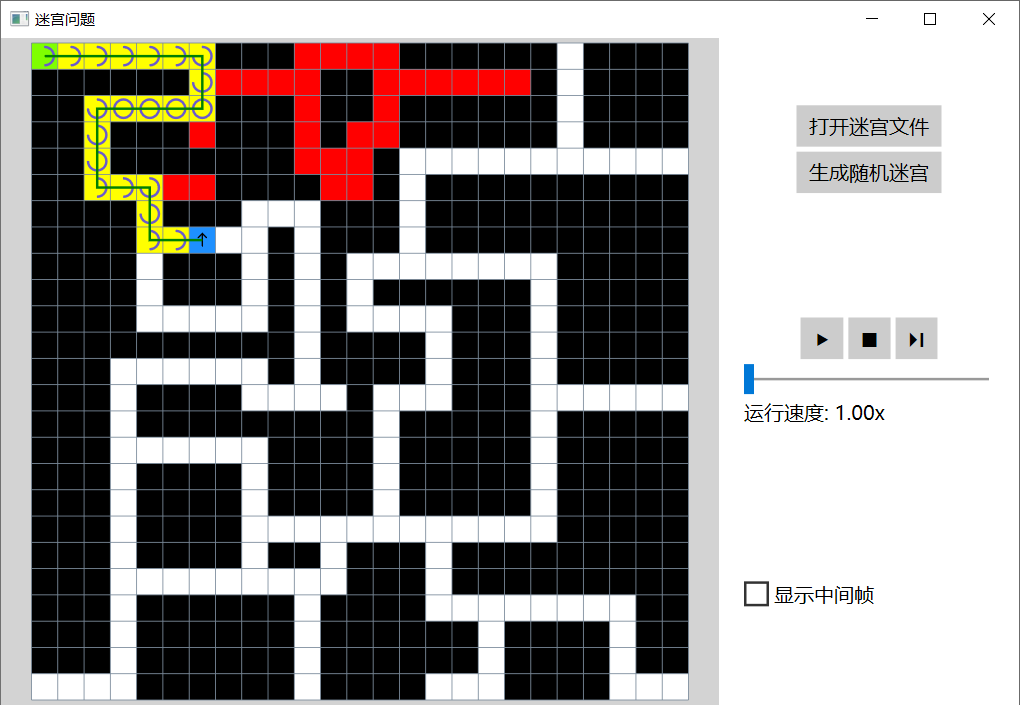
\includegraphics[width=\textwidth]{image05.png}\caption{迷宫求解成功}
\end{figure}
\begin{figure}[H]
\centering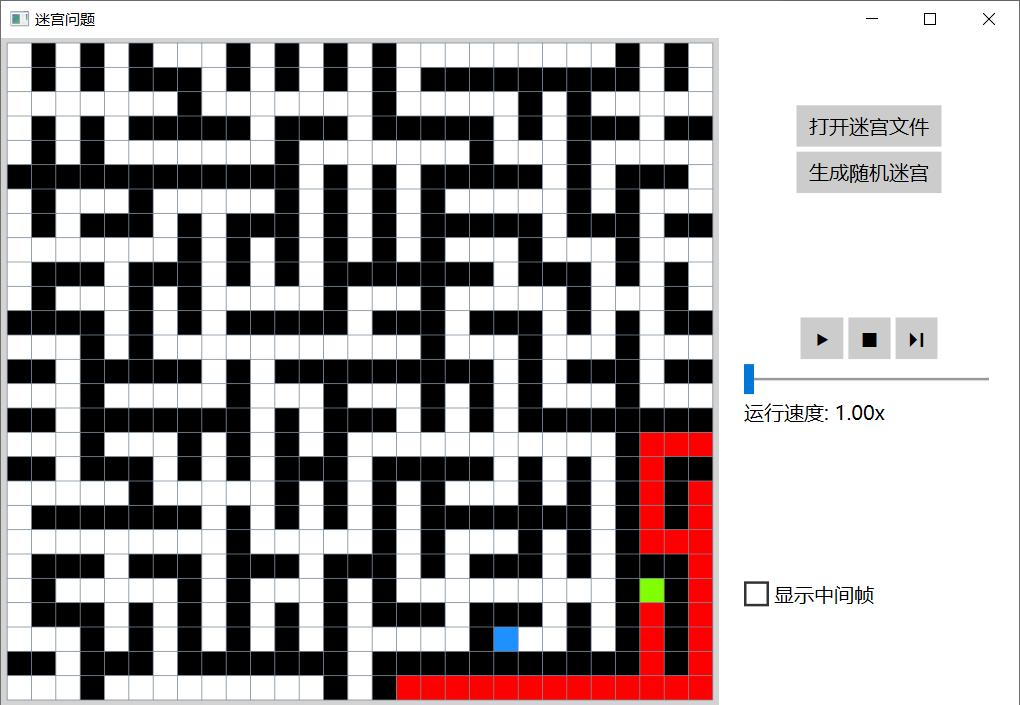
\includegraphics[width=\textwidth]{image06.png}\caption{迷宫求解失败}
\end{figure}
\subsection{时间复杂度}
时间复杂度为 $O(nm)$,其中 n、m 分别为迷宫的长、宽。
\subsection{问题及可改进的点}
迷宫的随机生成可以添加更多的随机性(如随机填充、加宽道路等)。

\section{B-树应用}
\subsection{数据结构}
使用的数据结构为 B-树。
\subsection{算法设计思想}
B-树的查找:从根节点开始搜索,寻找大于等于欲查找值的元素,若相等则输出,否则转至对应位置的子树继续搜索,直到到达叶子节点,寻找失败。\par
B-树的插入:类似查找过程,若相等则不做任何事,否则在叶子结点处有序插入给定的元素,若插入后结点大小超限则分裂当前结点为左结点、右结点、中间元素三者,将新增的结点及元素插入父亲结点,若分裂则重复之前的操作(若根节点分裂,则让中间元素单独成为新的父亲结点)。\par
B-树的删除:找到元素在树中的位置,若为非叶子结点则从子树中找到最接近的元素(如左子树的最右侧元素),移动上去,从而转换为从叶子结点中删除元素。若删除后结点元素超出下限,则尝试从兄弟结点借元素(将兄弟结点的一侧元素与父亲结点中所对应的元素“旋转”至当前结点),若兄弟结点也没有足够的元素,则执行分裂的逆操作(将左、右结点及父亲结点中所对应的元素合并为新的父亲的孩子结点)(若合并后根节点为空,则删去根节点)。
\subsection{源程序}
\cppcode{../代码/19-B-树应用/main.cpp}
{\captionof{listing}{main.cpp}}
源代码 json.h、json.cpp、hashmap.h、hashmap.cpp 可分别见本报告中的代码 2、3、4、5。
\subsection{测试数据及结果}
可能的交互如下:
\textcode{./interactions/19-01.txt}
\subsection{时间复杂度}
三种操作的时间复杂度均为 $O(\log n)$。
\subsection{问题及可改进的点}
可以尝试对代码进行更好的规划,进一步增强代码可维护性。

\section{总结}
\subsection{总体完成情况及代码行数}
基本上完成了所有的必做题要求与总分值为 14 的六道选做题,代码行数如下表所示(不包括空行、注释、完全重复的文件):
\begin{table}[H]
\centering
\begin{tabular}{|l|l|}
    \hline
    菜鸟智慧系统 & 1628 \\
    \hline
    算术表达式求值 & 382 \\
    \hline
    特殊路径统计 & 70 \\
    \hline
    公交线路提示 & 339 \\
    \hline
    Huffman 编码与解码 & 474 \\
    \hline
    排序算法比较 & 387 \\
    \hline
    棋局评估 & 82 \\
    \hline
    URL 映射 & 164 \\
    \hline
    词梯 & 246 \\
    \hline
    连连看 & 1622 \\
    \hline
    迷宫问题 & 2917 \\
    \hline
    B-树应用 & 638 \\
    \hline
    总计 & 8949 \\
    \hline
\end{tabular}
\end{table}
\subsection{心得体会}
这次课程设计的工作量总体来说还是不少的,也尝试结合了一些课外的东西。如第一题中为了保证存储数据在清晰、直观的前提下仍然易于处理,我选择了在两者中取得平衡的 JSON 格式,并花费了数天时间完成了相关处理的代码;为了实现高效的链表排序,我根据课外资料编写了自底向上的归并排序算法,等等。编写课设的过程中,由于疫情原因,本来是当学期就要完成的工作被迫拖到了下学期,但多出来的时间恰好给了我一个去实践更大胆、新颖的想法的契机。连连看、迷宫问题这两个具有图形界面的项目便成为了我实践一些个人想法的平台,虽然中间过程掉了许多坑、花费了数周时间去完成,最终的效果与题目的要求也没有什么关联,但光是成功地达成了我预期的效果这一点就足以令我心满意足了。这次的课设充分地锻炼了我的编程能力,更深入地理解、巩固了课程所学知识,体验了将理论知识投入实践的操作与意义,总的来说收获颇丰。

\end{document}
